\documentclass{article}

% packages
\usepackage{amsmath, amsthm, thmtools, amsfonts, amssymb, luacode, catchfile, tikzducks, hyperref, ifthen}
\ifcsname c@kobocompile\endcsname
	\usepackage[a5paper, total={1072pt, 1448pt}, margin=10pt, includeheadfoot]{geometry} % set page margins
\else
	\usepackage[a4paper, margin=50pt, includeheadfoot]{geometry}
\fi
\usepackage[shortlabels]{enumitem}
\usepackage[skip=3pt, indent=0pt]{parskip}

% language
\usepackage[bidi=basic, layout=tabular, provide=*]{babel}
\ifcsname c@english\endcsname
	\babelprovide[main, import]{english}
\else
	\babelprovide[main, import]{hebrew}
	\babelprovide{rl}
\fi
%\babelfont{rm}{Libertinus Serif}
\babelfont{rm}[Renderer=Harfbuzz]{Libertinus Serif}
\babelfont{sf}{Libertinus Sans}
\babelfont{tt}{Libertinus Mono}

% style
\AddToHook{cmd/section/before}{\clearpage}	% Add line break before section
\linespread{1.3}
\setcounter{secnumdepth}{0}		% Remove default number tags from sections, this won't do well with theorems
\AtBeginDocument{\setlength{\belowdisplayskip}{3pt}}
\AtBeginDocument{\setlength{\abovedisplayskip}{3pt}}
\graphicspath{ {../images/} }

% operators
\DeclareMathOperator\cis{cis}
\DeclareMathOperator\Sp{Sp}
\DeclareMathOperator\tr{tr}
\DeclareMathOperator\im{Im}
\DeclareMathOperator\re{Re}
\DeclareMathOperator\diag{diag}
\DeclareMathOperator*\lowlim{\underline{lim}}
\DeclareMathOperator*\uplim{\overline{lim}}
\DeclareMathOperator\rng{rng}
\DeclareMathOperator\Sym{Sym}
\DeclareMathOperator\Arg{Arg}
\DeclareMathOperator\Log{Log}
\DeclareMathOperator\dom{dom}
\DeclareMathOperator\supp{Supp}
\DeclareMathOperator\var{Var}
\DeclareMathOperator\cov{Cov}

% commands
%\renewcommand\qedsymbol{\textbf{מש''ל}}
%\renewcommand\qedsymbol{\fbox{\emoji{lizard}}}
\newcommand{\Aa}[0]{\mathcal{A}}
\newcommand{\Bb}[0]{\mathcal{B}}
\newcommand{\CC}[0]{\mathbb{C}}
\newcommand{\Cc}[0]{\mathcal{C}}
\newcommand{\EE}[0]{\mathbb{E}}
\newcommand{\FF}[0]{\mathbb{F}}
\newcommand{\Ff}[0]{\mathcal{F}}
\newcommand{\Ii}[0]{\mathcal{I}}
\newcommand{\Gg}[0]{\mathcal{G}}
\newcommand{\Ll}[0]{\mathcal{L}}
\newcommand{\Mm}[0]{\mathcal{M}}
\newcommand{\NN}[0]{\mathbb{N}}
\newcommand{\Nn}[0]{\mathcal{N}}
\newcommand{\PP}[0]{\mathbb{P}}
\newcommand{\Pp}[0]{\mathcal{P}}
\newcommand{\QQ}[0]{\mathbb{Q}}
\newcommand{\RR}[0]{\mathbb{R}}
\newcommand{\Rr}[0]{\mathcal{R}}
\newcommand{\Ss}[0]{\mathcal{S}}
\newcommand{\TT}[0]{\mathbb{T}}
\newcommand{\Uu}[0]{\mathcal{U}}
\newcommand{\Vv}[0]{\mathcal{V}}
\newcommand{\Ww}[0]{\mathcal{W}}
\newcommand{\ZZ}[0]{\mathbb{Z}}
\newcommand{\acts}[0]{\circlearrowright}
\newcommand{\explain}[2] {
	\begin{flalign*}
		 && \text{#2} && \text{#1}
	\end{flalign*}
}
\newcommand{\maketitleprint}[0]{ \begin{center}
	%\begin{tikzpicture}[scale=3]
	%	\duck[graduate=gray!20!black, tassel=red!70!black]
	%\end{tikzpicture}	
	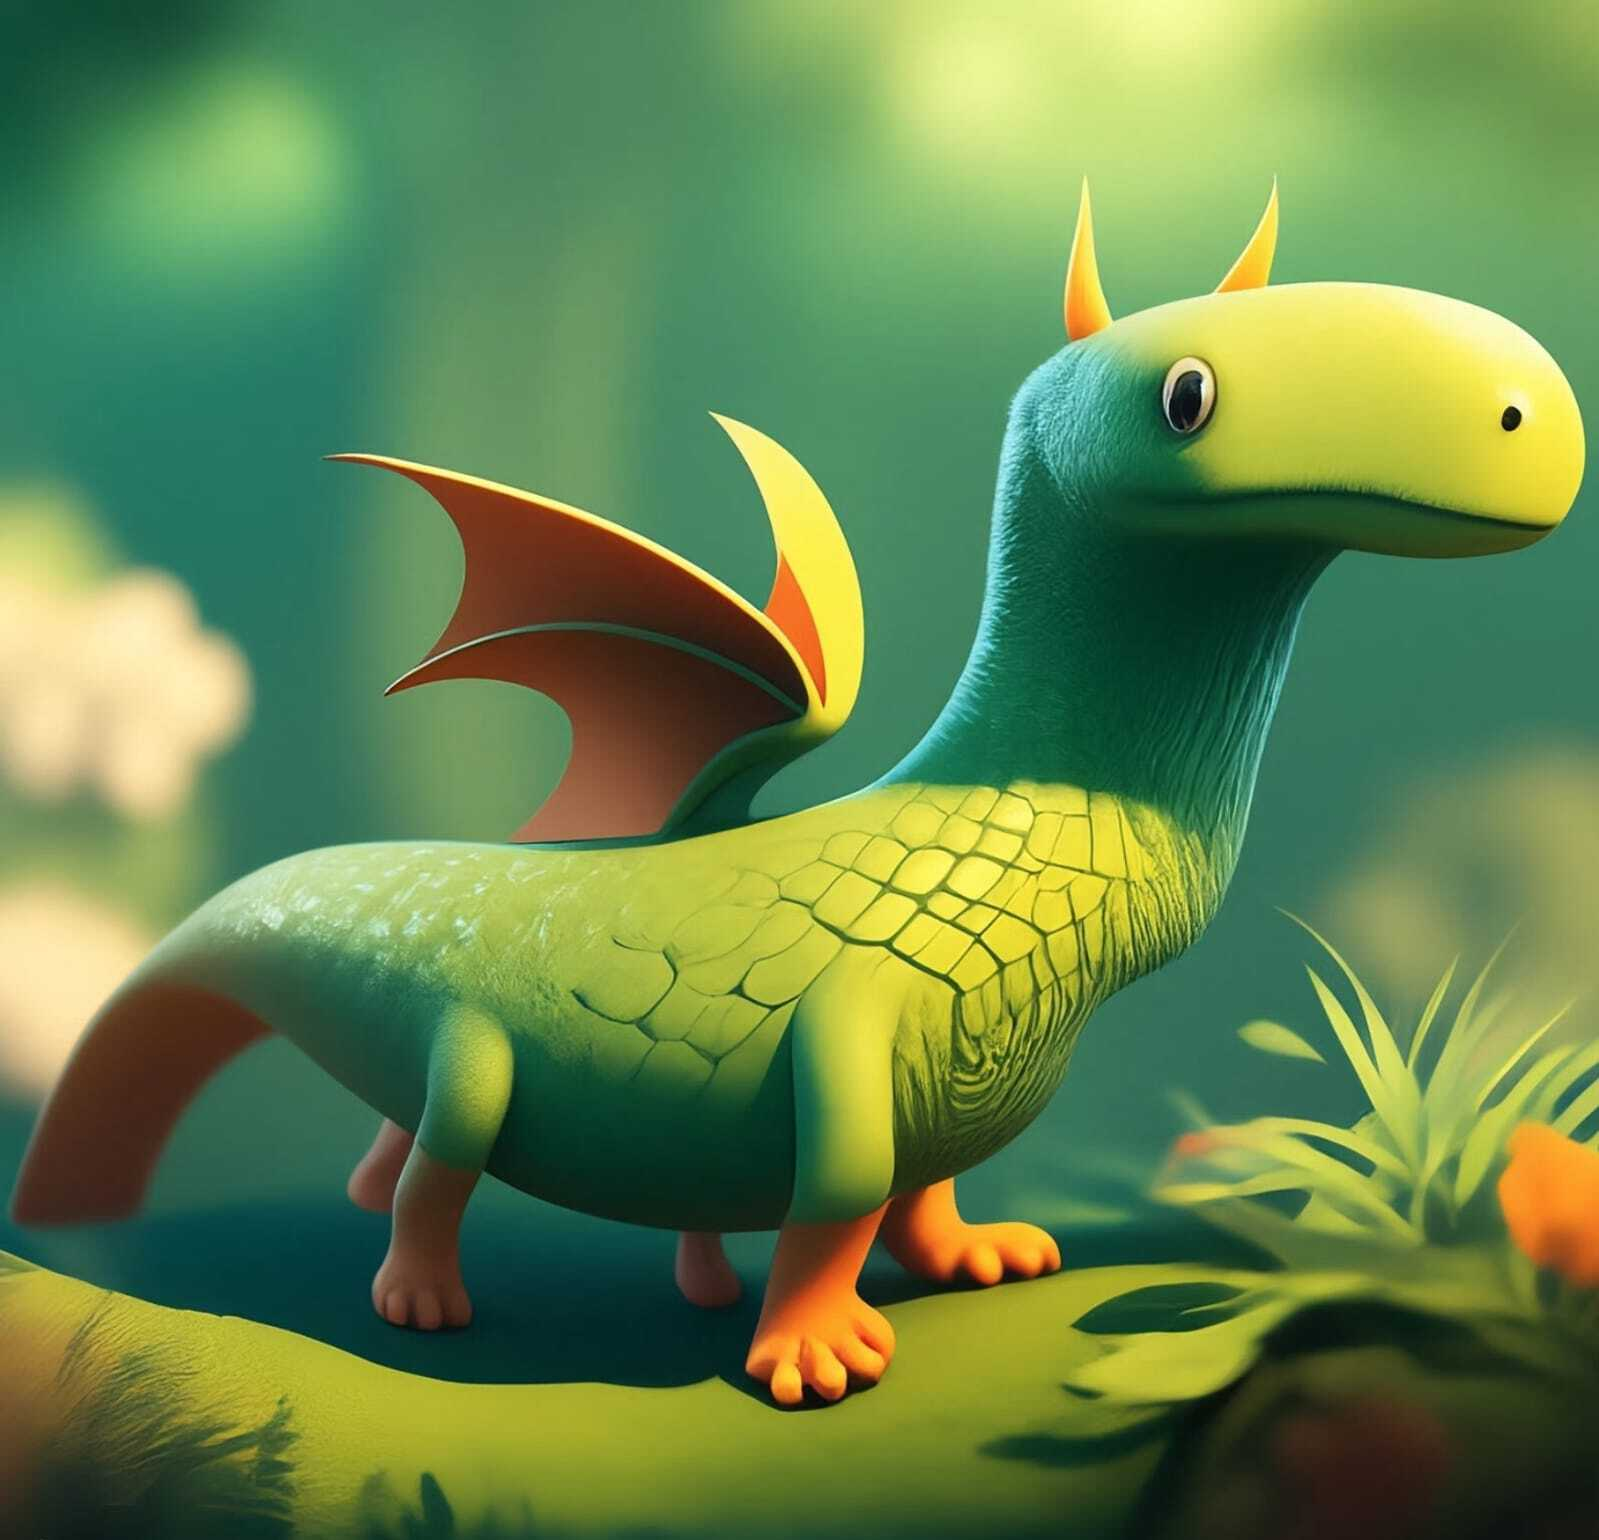
\includegraphics[width=6cm]{cover}
\end{center}
}

% theorem commands
\newtheoremstyle{c_remark}
	{}	% Space above
	{}	% Space below
	{}% Body font
	{}	% Indent amount
	{\bfseries}	% Theorem head font
	{}	% Punctuation after theorem head
	{.5em}	% Space after theorem head
	{\thmname{#1}\thmnumber{ #2}\thmnote{ \normalfont{\text{(#3)}}}}	% head content
\newtheoremstyle{c_definition}
	{3pt}	% Space above
	{3pt}	% Space below
	{}% Body font
	{}	% Indent amount
	{\bfseries}	% Theorem head font
	{}	% Punctuation after theorem head
	{.5em}	% Space after theorem head
	{\thmname{#1}\thmnumber{ #2}\thmnote{ \normalfont{\text{(#3)}}}}	% head content
\newtheoremstyle{c_plain}
	{3pt}	% Space above
	{3pt}	% Space below
	{\itshape}% Body font
	{}	% Indent amount
	{\bfseries}	% Theorem head font
	{}	% Punctuation after theorem head
	{.5em}	% Space after theorem head
	{\thmname{#1}\thmnumber{ #2}\thmnote{ \text{(#3)}}}	% head content

\ifcsname c@english\endcsname
	\theoremstyle{plain}
	\newtheorem{theorem}{Theorem}[section]
	\newtheorem{lemma}[theorem]{Lemma}
	\newtheorem{proposition}[theorem]{Proposition}
	\newtheorem*{proposition*}{Proposition}
	%\newtheorem{corollary}[theorem]{אין חלופה עברית}

	\theoremstyle{definition}
	\newtheorem{definition}[theorem]{Definition}
	\newtheorem*{definition*}{Definition}
	\newtheorem{example}{Example}[section]
	\newtheorem{exercise}{Exercise}[section]

	\theoremstyle{remark}
	\newtheorem*{remark}{Remark}
	\newtheorem*{solution}{Solution}
	\newtheorem{conclusion}[theorem]{Conclusion}
	\newtheorem{notation}[theorem]{Notation}
\else
	\theoremstyle{c_plain}
	\newtheorem{theorem}{משפט}[section]
	\newtheorem{lemma}[theorem]{למה}
	\newtheorem{proposition}[theorem]{טענה}
	\newtheorem*{proposition*}{טענה}
	%\newtheorem{corollary}[theorem]{אין חלופה עברית}

	\theoremstyle{c_definition}
	\newtheorem{definition}[theorem]{הגדרה}
	\newtheorem*{definition*}{הגדרה}
	\newtheorem{example}{דוגמה}[section]
	\newtheorem{exercise}{תרגיל}[section]

	\theoremstyle{c_remark}
	\newtheorem*{remark}{הערה}
	\newtheorem*{solution}{פתרון}
	\newtheorem{conclusion}[theorem]{מסקנה}
	\newtheorem{notation}[theorem]{סימון}
\fi

% Questions related commands
\newcounter{question}
\setcounter{question}{1}
\newcounter{sub_question}
\setcounter{sub_question}{1}

\ifcsname c@english\endcsname
	\newcommand{\question}[1][0]{
		\ifthenelse{#1 = 0}{}{\setcounter{question}{#1}}
		\section{Question \arabic{question}}
		\addtocounter{question}{1}
		\setcounter{sub_question}{1}
	}

	\newcommand{\subquestion}[1][0]{
		\ifthenelse{#1 = 0}{}{\setcounter{sub_question}{#1}}
		\subsection{Part \alph{sub_question}}
		\addtocounter{sub_question}{1}
	}
\else
	\newcommand{\question}[1][0]{
		\ifthenelse{#1 = 0}{}{\setcounter{question}{#1}}
		\section{שאלה \arabic{question}}
		\addtocounter{question}{1}
		\setcounter{sub_question}{1}
	}

	\newcommand{\subquestion}[1][0]{
		\ifthenelse{#1 = 0}{}{\setcounter{sub_question}{#1}}
		\subsection{סעיף \localecounter{letters.gershayim}{sub_question}}
		\addtocounter{sub_question}{1}
	}
\fi

% import lua and start of document
\directlua{common = require ('../common')}

\GetEnv{AUTHOR}

% headers
\author{\AUTHOR}
\date\today

\title{פתרון מטלה 02 --- פונקציות מרוכבות, 80519}

\begin{document}
\maketitle
\maketitleprint{}

\Question{}
תהינה $f, g : U \to \CC$ פונקציות אנליטיות המוגדרות על קבוצה פתוחה $U \subseteq \CC$.

\Subquestion{}
נוכיח כי $(f + g)'(z) = f'(z) + g'(z)$.
\begin{proof}
	מהגדרת הנגזרת נובע
	\[
		(f + g)'(z_0)
		= \lim_{z \to z_0} \frac{(f + g)(z) - (f + g)(z_0)}{z - z_0}
		= \lim_{z \to z_0} \frac{f(z) - f(z_0)}{z - z_0} + \frac{g(z) - g(z_0)}{z - z_0}
	\]
	אבל שני הביטויים הללו נתונים ולכן מאריתמטיקה
	\[
		(f + g)'(z_0)
		= \lim_{z \to z_0} \frac{f(z) - f(z_0)}{z - z_0} + \lim_{z \to z_0}  \frac{g(z) - g(z_0)}{z - z_0}
		= f'(z_0) + g'(z_0)
	\]
\end{proof}

\Subquestion{}
נוכיח כי $(f \cdot g)'(z) = f'(z) g(z) + f(z) g'(z)$.
\begin{proof}
	מהגדרת הנגזרת ומרציפות פונקציות גזירות נובע
	\begin{align*}
		(f \cdot g)'(z_0)
		& = \lim_{z \to z_0} \frac{(f \cdot g)(z) - (f \cdot g)(z_0)}{z - z_0} \\
		& = \lim_{z \to z_0} \frac{f(z) \cdot g(z) - f(z_0) \cdot g(z_0)}{z - z_0} \\
		& = \lim_{z \to z_0} \frac{(f(z) - f(z_0)) \cdot g(z) + f(z_0) g(z) - f(z_0) \cdot g(z_0)}{z - z_0} \\
		& = \lim_{z \to z_0} \frac{f(z) - f(z_0)}{z - z_0} \cdot g(z) + \frac{f(z_0) g(z) - f(z_0) \cdot g(z_0)}{z - z_0} \\
		& = f'(z_0) g(z_0) + f(z_0) \lim_{z \to z_0} \frac{g(z) - g(z_0)}{z - z_0} \\
		& = f'(z_0) g(z_0) + f(z_0) g'(z_0)
	\end{align*}
\end{proof}

\Subquestion{}
נוכיח כי $(f \circ g)'(z) = f'(g(z)) \cdot g'(z)$.
\begin{proof}
	מהגדרת הנגזרת נקבל
	\begin{align*}
		(f \circ g)'(z_0)
		& = \lim_{z \to z_0} \frac{(f \circ g)(z) - (f \circ g)(z_0)}{z - z_0} \\
		& = \lim_{z \to z_0} \frac{f(g(z)) - f(g(z_0))}{g(z) - g(z_0)} \cdot \frac{g(z) - g(z_0)}{z - z_0} \\
		& = f'(g(z_0)) \cdot g'(z_0)
	\end{align*}
\end{proof}

\Question{}
עבור הפונקציות הבאות נמצא את נקודות הגזירות ונקבע באילו נקודות היא אנליטית.

\Subquestion{}
\[
	f(x + iy) = (x^2 + y^2) + i (-x^2 + y^2)
\]
\begin{solution}
	נבחין כי אם נגזור את החלק מממשי נקבל
	\[
		\re(f(x + iy))' = (x^2 + y^2)' = (2x, 2y)
	\]
	ובאופן דומה
	\[
		\im(f(x + iy))' = (-x^2 + y^2)' = (-2x, 2y)
	\]
	כמובן $2y = 2y$ בכל התחום, אך $2x = - 2x \iff x = 0$ ולכן היא גזירה על הציר המדומה בלבד. \\*
	בהתאם אין נקודה פנימית בתחום הגזירות ולכן $f$ לא אנליטית לאף נקודה.
\end{solution}

\Subquestion{}
\[
	g(x + iy) = x^2 + 3iy
\]
גם הפעם נחשב
\[
	\re(g(x + iy))' = (3x^2, 0),
	\qquad
	\im(g(x + iy))' = (0, 3)
\]
אין נקודה בה $3 = 0$ ולכן $g$ לא גזירה באף נקודה.

\Subquestion{}
\[
	h(x + iy) = |x^2 - y^2| + 2i xy
\]
\begin{solution}
	נבחן את הנגזרות החלקיות כשאר $x^2 \ge y^2$:
	\[
		\re(h)' = (2x , -2y),
		\qquad
		\im(h)' = (2, 2)
	\]
	ונקבל גזירות כאשר $x = 1, y = -1$ בלבד. \\*
	נבחן את הנגזרות החלקיות בשאר המקרים:
	\[
		\re(h)' = (-2x, 2y),
		\qquad
		\im(h)' = (2, 2)
	\]
	ונקבל $x = -1, y = 1$ בלבד, אך לא מתקיים ${(-1)}^2 < 1^2$ ולכן נוכל להסיק כי $1 - i$ נקודת גזירות יחידה.
\end{solution}

\Subquestion{}
\[
	\forall a, b \in \CC,
	k(z) = az + b \overline{z}
\]
\begin{solution}
	ראינו כבר כי אם $b = 0$ אז $k$ גזירה ואנליטית בכל תחומה. \\*
	אילו $a = 0$ נקבל
	\[
		\lim_{z \to z_0} b\frac{\overline{z} - \overline{z_0}}{z - z_0}
		= b \lim_{z \to z_0} \frac{\overline{z - z_0}}{z - z_0}
	\]
	ומכאן ניתן לראות כי הצבה של סדרות ממשיות תניב נגזרת $1$ והצבת סדרות מדומות תניב $-1$ ו־$k$ איננה גזירה באף נקודה. \\*
	נניח $a, b \ne 0$ ונניח שקיימים ערכים עבורם $k$ גזירה, נקבל אם כך $(a z + b \overline{z})'$ גזיר, ומשאלה 1 נסיק $az' + b\overline{z}'$ ביטוי מוגדר, וזו כמובן סתירה לתוצאה שקיבלנו זה עתה. \\*
	נסיק שכל עוד $b = 0$ אז $k$ הולומורפית.
\end{solution}

\Question{}
תהי $f : G \to \CC$ פונקציה אנליטית המוגדרת על תחום $G \subseteq \CC$.

\Subquestion{}
נוכיח כי אם $\forall z \in G, f'(z) = 0$ אז $f$ בהכרח קבועה.
\begin{proof}
	תהינה שתי נקודות $z_0, z_1 \in G$, נניח גם $z_0 \ne z_1$. \\*
	נגדיר מסילה $l = [z_0, z_1]$, אז כמובן $l : \RR \to \CC$, ונבחן את הגרסה שלה בשני משתנים $l : \RR \to \RR^2$ במקום. \\*
	בגרסה זו נגזרתה מתלכדת עם הנגזרת הכיוונית $Df_{z_1 - z_0} = 0$, ולכן גם $\nabla l = {(0, 0)}^t$. \\*
	ידוע ש־$z_0 \ne z_1 \iff (\re(z_0) \ne \re(z_1) \lor \im(z_0) \ne \im(z_1))$ נניח בלי הגבלת הכלליות ש־$\re(z_0) \ne \re(z_1)$ ולכן אם $l = (l_1, l_2)$ מספיק שנבחן את $l_1$. \\*
	קיבלנו ש־$l_1 : \RR \to \RR$ וגם $l'(t) = 0$ לכל $0 \le t \le 1$, ולכן $l_1(0) = l_1(1)$ וזאת בסתירה להנחתנו, לכן $z_0 = z_1$ בלבד.
\end{proof}

\Subquestion{}
נוכיח כי אם $f(G) \subseteq \RR$ אז $f$ בהכרח קבועה.
\begin{proof}
	נראה כי אם $z = x + iy$ אז נובע
	\[
		\frac{\partial f}{\partial x} (x_0 + iy_0) = \frac{\partial f}{\partial iy} (x_0 + iy_0) = 0
	\]
	דהינו $f$ אנליטית אם ורק אם $f'(z) = 0$ לכל $z \in G$, אז מהסעיף הקודם נובע $f$ קבועה.
\end{proof}

\Subquestion{}
נוכיח כי אם $f(\overline{z})$ אנליטית אז $f$ בהכרח קבועה.
\begin{proof}
	מנתון נסיק ישירות כי גם $\overline{f(\overline{\overline{z}})}$ אנליטית, דהינו $\overline{f(z)}$. \\*
	אבל ידוע כי גם $f$ גזירה ולכן
	\[
		\frac{\partial f}{\partial iy}(z)
		= \frac{\partial f}{\partial x}(z)
		= \frac{\partial \overline{f}}{\partial x}(z)
		= \frac{\partial \overline{f}}{\partial iy}(z)
		= -\frac{\partial f}{\partial iy}(z)
	\]
	ולכן $\frac{\partial f}{\partial iy}(z) = 0$ בלבד, ולכן $f'(z) = 0$ לכל $z \in G$, אז מסעיף א' היא קבועה.
\end{proof}

\Subquestion{}
נוכיח כי $\overline{f(\overline{z})}$ אנליטית ונחשב את ערכה.
\begin{proof}
	\begin{align*}
		\lim_{z \to z_0} \frac{\overline{f(\overline{z})} - \overline{f(\overline{z_0})}}{z - z_0}
		& = \lim_{z \to z_0} \frac{\overline{f(\overline{z}) - f(\overline{z_0})}}{z - z_0} \\
		& = \lim_{z \to z_0} \frac{\overline{z - z_0}}{{|z - z_0|}^2} (\overline{f(\overline{z}) - f(\overline{z_0})}) \\
		& = \lim_{z \to z_0} \frac{1}{{|z - z_0|}^2} \overline{(f(\overline{z}) - f(\overline{z_0})) (z - z_0)} \\
		& = \lim_{z \to z_0} \overline{\left(\frac{f(\overline{z}) - f(\overline{z_0})}{\overline{z} - \overline{z_0}}\right)} \\
		& = \overline{\left(\lim_{z \to z_0} \frac{f(\overline{z}) - f(\overline{z_0})}{\overline{z} - \overline{z_0}}\right)} \\
		& = \overline{f'(\overline{z})}
	\end{align*}
\end{proof}

\Question{}
נחשב את החלק הממשי, החלק מהדומה, הערך המוחלט ואת השורשים של הפונקציות הנתונות.

\Subquestion{}
נבחן את $\cos(z)$.
\begin{solution}
	תחילה נמצא ביטוי בערך ממשי ומדומה לביטוי:
	\begin{align*}
		\cos(x + iy)
		& = \frac{1}{2}(e^{i(x + iy)} + e^{-i(x + iy)}) \\
		& = \frac{1}{2}(e^{ix} e^{-y} + e^{-ix} e^{y}) \\
		& = \frac{1}{2}((\cos(x) + i\sin(x)) e^{-y} + (\cos(-x) + i\sin(-x)) e^{y}) \\
		& = \frac{1}{2}(\cos(x) e^{-y} + \cos(x) e^{y}) + i \frac{1}{2}(\sin(x) e^{-y} - \sin(x) e^{y})
	\end{align*}
	נעבור לחישוב הערך המוחלט:
	\begin{align*}
		|\cos(x + iy)|
		& = \sqrt{{(\frac{1}{2}(\cos(x) e^{-y} + \cos(x) e^{y}))}^2 + {(\frac{1}{2}(\sin(x) e^{-y} - \sin(x) e^{y}))}^2} \\
		& = \sqrt{\frac{1}{4} ( {(\cos(x) e^{-y} + \cos(x) e^{y})}^2 + {(\sin(x) e^{-y} - \sin(x) e^{y})}^2 )} \\
		& = \sqrt{\frac{1}{4} (\cos^2(x) e^{-2y} + 2\cos^2(x) + \cos^2(x)e^{2y} + \sin^2(x) e^{-2y} - 2\sin^2(x) + \sin^2(x)e^{2y})} \\
		& = \frac{1}{2} \sqrt{e^{-2y} + e^{2y} + 2\cos(2x)}
	\end{align*}
	לבסוף נבדוק את השורשים על־ידי שימוש בזהות $\cos(z) = 0 \iff |\cos(z)| = 0$, דהינו
	\[
		\frac{1}{2} \sqrt{e^{-2y} + e^{2y} + 2\cos(2x)} = 0
		\iff e^{-2y} + e^{2y} + 2\cos(2x) = 0
		\iff \cos(2x) = \frac{e^{2y} + e^{-2y}}{2}
	\]
	אבל כמובן אם $y \ne 0$ נקבל ביטוי קטן מ־$-1$ ולכן $y = 0$, ו־$\cos(2x) = -1$, דהינו $x = \frac{\pi}{2} + \pi k$.
\end{solution}

\Subquestion{}
נעבור לבדוק את $\sin(z)$.
\begin{solution}
	ידוע כי $\sin(z) = \frac{e^{iy} - e^{-iy}}{2i}$, לכן נבצע אותו הליך שעשינו בסעיף הקודם תוך התחשבות בשינוי הסימן ונסיק
	\begin{align*}
		\sin(x + iy)
		& = \frac{1}{2i}(\cos(x) e^{-y} - \cos(x) e^{y}) + i \frac{1}{2i}(\sin(x) e^{-y} + \sin(x) e^{y}) \\
		& = \frac{1}{2}(\sin(x) e^{-y} + \sin(x) e^{y}) + i\frac{1}{2}(\cos(x) e^{y} - \cos(x) e^{-y})
	\end{align*}
	הערך המוחלט הוא:
	\begin{align*}
		|\sin(x + iy)|
		& = \frac{1}{2} \sqrt{\sin^2(x) (e^{-2y} + 2 + e^{2y}) + \cos^2(x) (e^{y} - 2 + e^{-y})} \\
		& = \frac{1}{2} \sqrt{e^{-2y} + e^{2y} - 2\cos(2x) }
	\end{align*}
	לבסוף נקבל שהשורשים הם $z = \pi k$ משיקולים זהים לסעיף הקודם.
\end{solution}

\Subquestion{}
נחקור את $\tan(z)$:
\begin{solution}
	נתחיל בחישוב החלק השלם והמדומה על־ידי שימוש בסעיפים הקודמים:
	\begin{align*}
		\tan(x + i y)
		& = \frac{\frac{1}{2}(\sin(x) e^{-y} + \sin(x) e^{y}) + i\frac{1}{2}(\cos(x) e^{y} - \cos(x) e^{-y})}{\frac{1}{2}(\cos(x) e^{-y} + \cos(x) e^{y}) + i \frac{1}{2}(\sin(x) e^{-y} - \sin(x) e^{y})} \\
		& = \frac{(\sin(x) (e^{-y} + e^{y}) + i \cos(x) (e^{y} - e^{-y}))(\cos(x) (e^{-y} + e^{y}) - i \sin(x) (e^{-y} - e^{y}))}{e^{-2y} + e^{2y} + 2\cos(2x)} \\
		& = \frac{\sin(x)\cos(x)({(e^y + e^{-y})}^2 - {(e^y - e^{-y})}^2) + i( \sin^2(x)(e^{2y} - e^{-2y}) + \cos^2(x) (e^{2y} - e^{-2y}) )}{e^{-2y} + e^{2y} + 2\cos(2x)} \\
		& = \frac{2\sin(2x) + i(e^{2y} - e^{-2y})}{2\cos(2x) + e^{2y} + e^{-2y}} \\
	\end{align*}
	נעבור לחישוב הערך המוחלט:
	\[
		|\tan(x + iy)|
		= \frac{\sqrt{4\sin^2(2x) + {(e^{2y} - e^{-2y})}^2}}{2\cos(2x) + e^{2y} + e^{-2y}} \\
	\]
	ושורשים כבר חישבנו, שכן $\tan(z)$ מתאפס אם ורק אם $\sin(z)$ מתאפס מהגדרה.
\end{solution}

\Question{}
יהיו $z, w \in \CC$.

\Subquestion{}
נוכיח כי $\cos^2(z) + \sin^2(z) = 1$.
\begin{proof}
	\[
		\cos^2(z) + \sin^2(z)
		= \frac{e^{-2z} + 2 e^{0} + e^{-2z}}{4} + \frac{e^{-2z} - 2 e^{0} + e^{2z}}{-4}
		= 1
	\]
\end{proof}

\Subquestion{}
נוכיח כי $\sin(z + w) = \sin(z) \cos(w) + \cos(z) \sin(w)$.
\begin{proof}
	נחשב
	\begin{align*}
		\sin(z + w)
		& = \frac{1}{2i}(e^{i(z + w)} - e^{-i(z + w)}) \\
		& = \frac{1}{2i}(e^{iz} e^{iw} - e^{-iz} e^{-iw}) \\
		& = \frac{1}{4i}(e^{iz} e^{iw} - e^{-iz} e^{iw} + e^{iz} e^{-iw} - e^{-iz} e^{-iw} + e^{iz} e^{iw} + e^{-iz} e^{iw} - e^{iz} e^{-iw} - e^{-iz} e^{-iw}) \\
		& = \frac{1}{4i}(e^{iz} - e^{-iz})(e^{iw} + e^{-iw}) + \frac{1}{4i}(e^{iz} + e^{-iz})(e^{iw} - e^{-iw}) \\
		& = \sin(z) \cos(w) + \cos(z) \sin(w)
	\end{align*}
\end{proof}

\Subquestion{}
נוכיח את הזהות $\cos(3z) = 4\cos^3(z) - 3 \cos(z)$.
\begin{proof}
	נסמן $a = e^{iz}, b = e^{-iz}$, ונבחין כי $ab = e^{iz - iz} = 1$.
	נשתמש בהגדרת הטריגונומטריות המרוכבות
	\begin{align*}
		4\cos^3(z) - 3 \cos(z)
		& = 4 \frac{{(a + b)}^3}{2^3} - 3 \frac{a + b}{2} \\
		& = \frac{a^3 + 3 a^2 b + 3 a b^2 + b^3 - 3a - 3b}{2} \\
		& = \frac{a^3 + 3 a + 3 b + b^3 - 3a - 3b}{2} \\
		& = \frac{e^{i 3z} + e^{-i 3z}}{2} \\
		& = \cos(3z)
	\end{align*}
\end{proof}

\Question{}
נמצא את כל הנקודות $z \in \CC$ עבורן $\sum_{n = 0}^\infty \frac{z^{3n + 1}}{3n + 1}$ מתכנס.
\begin{solution}
	נגדיר ${(a_n)}_{n = 1}^\infty \subseteq \RR$ על־ידי
	\[
		a_n = \begin{cases}
			\frac{1}{3n + 1} & n \equiv 1 (\mod 3) \\
			0 & \text{else}
		\end{cases}
	\]
	לכן נקבל
	\[
		\sum_{n = 0}^\infty a_n z^n
		= \sum_{n = 0}^\infty \frac{z^{3n + 1}}{3n + 1}
	\]
	אז נוכל להסיק ממבחן אבל כי הטור מתכנס עבור $z \in \overline{B}(0, 1) \setminus \{1\}$. \\*
	כמובן עבור $|z| > 1$ נוכל לראות כי הערך המוחלט של הטור מתבדר ולכן גם הטור עצמו.
\end{solution}

\Question{}
יהי $\sum_{n = 0}^\infty \alpha_n$ טור מרוכב מתכנס.

\Subquestion{}
נוכיח כי אם $|\Arg(\alpha_n)| \le \theta < \frac{\pi}{2}$ לכל $n \in \NN$ אז הטור מתכנס בהחלט.
\begin{proof}
	נתון כי $-\theta \le \Arg(\alpha_n) \le \theta$, לכן גם $0 < \cos(\theta) \le \cos(\Arg(\alpha_n)) \le 1$. \\*
	עוד נבחין כי $\sum_{n = 0}^\infty \re(\alpha_n)$ מתכנס מהנתון כי הטור המקורי מתכנס, אבל מאי־השוויון הקודם נובע $0 < \re(\alpha_n)$ ולכן $\sum_{n = 0}^{\infty} |\re(\alpha_n)|$ מתכנס אף הוא,
	מצאנו כי סדרת הערכים הממשיים מתכנסת בהחלט. \\*
	נרצה עוד להראות כי $|\im(\alpha_n)| \le C |\re(\alpha_n)|$ עבור איזשהו $C \in [0, 1]$. \\*
	נבחר $m = \sup_{n \in \NN} |\Arg(\alpha_n)|$, אז זהו גם האינפימום של $\cos(\Arg(\alpha_n))$,
	נגדיר $|\sin(\Arg(\alpha_m))| = C \cos(\Arg(\alpha_m))$ ולכן מהגדרה $|\sin(\Arg(\alpha_n))| \le C \cos(\Arg(\alpha_n))$ לכל $n \in \NN$.
	אבל אם כך אז $|\im(\alpha_n)| \le C \re(\alpha_n)$ לכל $n$ ובהתאם $\sum_{n = 0}^{\infty} |\im(\alpha_n)|$ מתכנס, דהינו מצאנו כי הן הערך הממשי והן הערך המדומה מתכנסים בהחלט, לכן גם $\sum_{n = 0}^{\infty} |\alpha_n|$ מתכנס.
\end{proof}

\Subquestion{}
נראה כי הטענה לא נכונה אם מניחים שרק $|\Arg(\alpha_n)| < \frac{\pi}{2}$ לכל $n \in \NN$ על־ידי דוגמה נגדית.
\begin{solution}
	נגדיר $\alpha_n = \frac{1}{n^2} + i {(-1)}^n \frac{1}{n}$. \\*
	לסדרה זו תמיד יש ערך ממשי חיובי ולכן היא מקיימת את תנאי הטענה. \\*
	נבחין כי $\re(\alpha_n) = \frac{1}{n^2} \to 0$ טור מתכנס בהחלט, וגם $\im(\alpha_n) = \frac{{(-1)}^n}{n}$ הוא טור לייבניץ ולכן נתכנס, ונקבל $\sum_{n = 1}^{\infty} \alpha_n$ מתכנס אף הוא. \\*
	לעומת זאת, מחישוב ישיר נקבל
	\[
		|\alpha_n| = \sqrt{\frac{1}{n^2} + \frac{1}{n^4}} = \frac{1}{n} \sqrt{1 + \frac{1}{n^2}}
	\]
	ולכן הטור של סדרה זו מתבדר כטור ממשי.
\end{solution}

\end{document}
